\documentclass[10pt,letterpaper,journal]{IEEEtran}
\usepackage{cite}
\usepackage{url}
\usepackage{graphicx}
\usepackage{booktabs}
\usepackage{pifont}
\usepackage{amssymb}
\usepackage{xcolor}
\usepackage{array}
\usepackage{tabularx}
\usepackage{amsmath}
\usepackage{amsthm}
\usepackage{newtxtext}
\usepackage{enumitem}
\usepackage{subcaption}
\usepackage{microtype}
\usepackage{xr}
% Cross-references into the main paper (\ref{M-label}); build.sh compiles it first
\externaldocument[M-]{build/ieee-paper}

\title{Supplementary Material: Constraint-Aware Zero-Knowledge Face Eligibility Against Lookalike Attackers: Sound Circuits and Attested Capture for Decentralized Voting}

\author{\IEEEauthorblockN{Mahin R. Chowdhury\IEEEauthorrefmark{1}\IEEEmembership{Student Member, IEEE},
K.~M.~Azharul Hasan\IEEEauthorrefmark{1}\IEEEmembership{Member, IEEE},
Arpita Das\IEEEauthorrefmark{1}\IEEEmembership{Student Member, IEEE}}
\IEEEauthorblockA{\IEEEauthorrefmark{1}Department of Computer Science and Engineering,\\
Khulna University of Engineering \& Technology,\\
Khulna-9203, Bangladesh\\
}}

\markboth{Supplementary Material for IEEE Transactions on Information Forensics and Security}{Chowdhury \emph{et al.}: Supplementary Material}

\newcommand{\vect}[1]{\mathbf{#1}}
% Generated by make_numbers.py from api-server/{benchmark,results}/*.json. Do not edit.
\newcommand{\nDim}{128}
\newcommand{\nTau}{0.35}
\newcommand{\nTauNum}{1{,}225}
\newcommand{\nLfwEer}{0.22}
\newcommand{\nLfwEerLo}{0.13}
\newcommand{\nLfwEerHi}{0.32}
\newcommand{\nFrr}{0.60}
\newcommand{\nFar}{0.013}
\newcommand{\nFalseAccepts}{26}
\newcommand{\nImpostorPairs}{200{,}000}
\newcommand{\nFacenetEer}{4.38}
\newcommand{\nFacenetEerLo}{4.02}
\newcommand{\nFacenetEerHi}{4.78}
\newcommand{\nCelebaEer}{4.02}
\newcommand{\nCelebaEerLo}{3.55}
\newcommand{\nCelebaEerHi}{4.49}
\newcommand{\nCelebaEmbedded}{39{,}726}
\newcommand{\nCelebaImages}{39{,}733}
\newcommand{\nMaleEer}{2.25}
\newcommand{\nMaleEerLo}{1.92}
\newcommand{\nMaleEerHi}{2.59}
\newcommand{\nFemaleEer}{5.10}
\newcommand{\nFemaleEerLo}{4.67}
\newcommand{\nFemaleEerHi}{5.69}
\newcommand{\nMaleIds}{878}
\newcommand{\nFemaleIds}{1{,}122}
\newcommand{\nGenderGap}{2.8}
\newcommand{\nGenderRatio}{2.3}
\newcommand{\nCelebaRawEer}{3.59}
\newcommand{\nFacenetCelebaEer}{8.09}
\newcommand{\nFacenetMaleEer}{7.93}
\newcommand{\nFacenetFemaleEer}{10.47}
\newcommand{\nDeepfaceEer}{6.10}
\newcommand{\nDeepfaceRatio}{46}
\newcommand{\nRawEer}{0.13}
\newcommand{\nInvCos}{0.72}
\newcommand{\nInvEer}{0.27}
\newcommand{\nInvRawEer}{0.13}
\newcommand{\nCalfwEer}{6.70}
\newcommand{\nCalfwEerLo}{5.88}
\newcommand{\nCalfwEerHi}{7.48}
\newcommand{\nCalfwRawEer}{6.47}
\newcommand{\nCalfwFrr}{9.6}
\newcommand{\nCalfwFar}{0.13}
\newcommand{\nCalfwUnseenFrr}{9.5}
\newcommand{\nCalfwImages}{7{,}156}
\newcommand{\nCalfwEmbedded}{7{,}156}
\newcommand{\nCplfwEer}{5.56}
\newcommand{\nCplfwEerLo}{4.93}
\newcommand{\nCplfwEerHi}{6.23}
\newcommand{\nCplfwRawEer}{4.65}
\newcommand{\nCplfwFrr}{13.8}
\newcommand{\nCplfwFar}{0.24}
\newcommand{\nCplfwUnseenFrr}{14.3}
\newcommand{\nCplfwImages}{5{,}984}
\newcommand{\nCplfwEmbedded}{5{,}950}
\newcommand{\nLookLfwOne}{0.004}
\newcommand{\nLookLfwTen}{0.10}
\newcommand{\nLookLfwHundred}{0.85}
\newcommand{\nLookLfwThousand}{8.4}
\newcommand{\nLookCelebaOne}{0.01}
\newcommand{\nLookCelebaTen}{0.16}
\newcommand{\nLookCelebaHundred}{1.7}
\newcommand{\nLookCelebaThousand}{14.1}
\newcommand{\nLookGenderOne}{0.03}
\newcommand{\nLookGenderTen}{0.21}
\newcommand{\nLookGenderHundred}{2.3}
\newcommand{\nLookGenderThousand}{25.6}
\newcommand{\nZeLookLfwOne}{0.10}
\newcommand{\nZeLookLfwTen}{0.97}
\newcommand{\nZeLookLfwHundred}{9.0}
\newcommand{\nZeLookLfwThousand}{59.6}
\newcommand{\nZeLookCelebaOne}{0.16}
\newcommand{\nZeLookCelebaTen}{1.4}
\newcommand{\nZeLookCelebaHundred}{13.3}
\newcommand{\nZeLookCelebaThousand}{71.1}
\newcommand{\nZeLookGenderOne}{0.20}
\newcommand{\nZeLookGenderTen}{1.8}
\newcommand{\nZeLookGenderHundred}{16.0}
\newcommand{\nZeLookGenderThousand}{83.7}
\newcommand{\nZeFrr}{0.47}
\newcommand{\nFaceConstraints}{32{,}668}
\newcommand{\nIrisConstraints}{17{,}518}
\newcommand{\nHashConstraints}{7{,}041}
\newcommand{\nCosConstraints}{5{,}656}
\newcommand{\nEuclidConstraints}{5{,}296}
\newcommand{\nMerkleConstraints}{4{,}840}
\newcommand{\nAttestConstraints}{7{,}368}
\newcommand{\nKeyMB}{30.9}
\newcommand{\nIrisKeyMB}{14.2}
\newcommand{\nAttestShare}{23}
\newcommand{\nPoseidonTwo}{240}
\newcommand{\nPackedHash}{1{,}905}
\newcommand{\nHamming}{778}
\newcommand{\nSigma}{5 \times 10^{5}}
\newcommand{\nCoordBits}{19}
\newcommand{\nTwoCoordBits}{38}
\newcommand{\nRangePerCoord}{20}
\newcommand{\nRangeConstraints}{5{,}120}
\newcommand{\nDotBits}{45}
\newcommand{\nCmpBits}{104}
\newcommand{\nDomainExp}{15}
\newcommand{\nHashSixteen}{1{,}044}
\newcommand{\nCosSixteen}{831}
\newcommand{\nFullCosSixteen}{15{,}849}
\newcommand{\nHashSixtyFour}{3{,}618}
\newcommand{\nCosSixtyFour}{2{,}901}
\newcommand{\nFullCosSixtyFour}{23{,}067}
\newcommand{\nHashNinetySix}{5{,}328}
\newcommand{\nCosNinetySix}{4{,}280}
\newcommand{\nFullCosNinetySix}{27{,}866}
\newcommand{\nHashOneSixty}{9{,}198}
\newcommand{\nCosOneSixty}{7{,}035}
\newcommand{\nFullCosOneSixty}{38{,}361}
\newcommand{\nHashTwoFiftySix}{14{,}322}
\newcommand{\nCosTwoFiftySix}{11{,}163}
\newcommand{\nFullCosTwoFiftySix}{52{,}737}
\newcommand{\nOneSixtyExtra}{17}
\newcommand{\nPerDim}{154}
\newcommand{\nEuclidSixtyFour}{2{,}672}
\newcommand{\nFullEuclidSixtyFour}{22{,}838}
\newcommand{\nFullEuclid}{32{,}308}
\newcommand{\nEuclidSaveSixtyFour}{229}
\newcommand{\nEuclidSave}{360}
\newcommand{\nMerkleMs}{53}
\newcommand{\nMerkleCi}{0.2}
\newcommand{\nEncryptMs}{83}
\newcommand{\nEncryptCi}{3}
\newcommand{\nWitnessMs}{209}
\newcommand{\nWitnessCi}{3}
\newcommand{\nProveMs}{1{,}345}
\newcommand{\nProveCi}{16}
\newcommand{\nClientMs}{1{,}690}
\newcommand{\nClientCi}{16}
\newcommand{\nSignMs}{27}
\newcommand{\nSignCi}{0.2}
\newcommand{\nVerifyMs}{19}
\newcommand{\nVerifyCi}{2}
\newcommand{\nCastVoteMs}{49}
\newcommand{\nCastVoteCi}{1}
\newcommand{\nProveShare}{80}
\newcommand{\nProveS}{1.35}
\newcommand{\nClientS}{1.7}
\newcommand{\nIrisProveS}{0.81}
\newcommand{\nIrisWitnessMs}{140}
\newcommand{\nIrisWitnessCi}{1}
\newcommand{\nIrisProveMs}{811}
\newcommand{\nIrisProveCi}{10}
\newcommand{\nIrisClientMs}{1{,}085}
\newcommand{\nIrisClientCi}{11}
\newcommand{\nIrisSignMs}{24}
\newcommand{\nIrisSignCi}{0.2}
\newcommand{\nIrisVerifyMs}{18}
\newcommand{\nIrisVerifyCi}{2}
\newcommand{\nIrisCastVoteMs}{49}
\newcommand{\nIrisCastVoteCi}{1}
\newcommand{\nScaleTenPathsMs}{4}
\newcommand{\nScaleTenProveMs}{1{,}368}
\newcommand{\nScaleTenCastMs}{49}
\newcommand{\nScaleThousandPathsMs}{52}
\newcommand{\nScaleThousandProveMs}{1{,}356}
\newcommand{\nScaleThousandCastMs}{49}
\newcommand{\nScaleFiveThousandPathsMs}{248}
\newcommand{\nScaleFiveThousandProveMs}{1{,}324}
\newcommand{\nScaleFiveThousandCastMs}{50}
\newcommand{\nScaleTwentyThousandPathsMs}{987}
\newcommand{\nScaleTwentyThousandProveMs}{1{,}368}
\newcommand{\nScaleTwentyThousandCastMs}{48}
\newcommand{\nScaleCastMin}{48}
\newcommand{\nScaleCastMax}{50}
\newcommand{\nScalePathsTopS}{1.0}
\newcommand{\nScalePathsMillionS}{49}
\newcommand{\nTallyVerifyMs}{27}
\newcommand{\nTallyPublishS}{0.43}
\newcommand{\nTallyMillionMin}{7}
\newcommand{\nTallyHundredVerifyS}{2.8}
\newcommand{\nTallyHundredDecryptMs}{28}
\newcommand{\nTallyHundredPublishMs}{68}
\newcommand{\nTallyThousandVerifyS}{27.4}
\newcommand{\nTallyThousandDecryptMs}{28}
\newcommand{\nTallyThousandPublishMs}{425}
\newcommand{\nFabVoters}{40}
\newcommand{\nFabInFlight}{10}
\newcommand{\nFabSeqS}{2.14}
\newcommand{\nFabConcS}{0.62}
\newcommand{\nFabTps}{16}
\newcommand{\nFabMillionH}{17}
\newcommand{\nFabRegisterS}{2.12}
\newcommand{\nFabPublishS}{2.23}
\newcommand{\nFabKeygenS}{10.4}
\newcommand{\nIrisProveShare}{75}
  % measured numbers, generated by make_numbers.py

\newtheorem{theorem}{Theorem}[section]
\newtheorem{lemma}[theorem]{Lemma}
\newtheorem{definition}[theorem]{Definition}
\newtheorem{proposition}[theorem]{Proposition}
\newtheorem{corollary}[theorem]{Corollary}
\newtheorem{remark}[theorem]{Remark}
\newtheorem{assumption}[theorem]{Assumption}

\newcommand{\cmark}{\textcolor{green!60!black}{\ding{51}}}
\newcommand{\pmark}{\textcolor{orange}{\textbf{$\sim$}}}
\newcommand{\xmark}{\textcolor{red}{\ding{55}}}

\setlength{\textfloatsep}{4pt plus 1pt minus 1pt}
\setlength{\floatsep}{3pt plus 1pt minus 1pt}
\setlength{\intextsep}{4pt plus 1pt minus 1pt}
\setlength{\dbltextfloatsep}{4pt plus 1pt minus 1pt}
\setlength{\dblfloatsep}{3pt plus 1pt minus 1pt}
\setlength{\abovecaptionskip}{2pt plus 0.5pt minus 0.5pt}
\setlength{\belowcaptionskip}{0pt}

\setlist{nosep,leftmargin=*,topsep=1pt,partopsep=0pt,parsep=0pt,itemsep=1pt}

\AtBeginDocument{
  \setlength{\abovedisplayskip}{3pt plus 1pt minus 1pt}
  \setlength{\belowdisplayskip}{3pt plus 1pt minus 1pt}
  \setlength{\abovedisplayshortskip}{1pt plus 0.5pt}
  \setlength{\belowdisplayshortskip}{1pt plus 0.5pt}
}

\begin{document}

\maketitle

% S-prefixed numbering so supplement floats never collide with the main paper's
\renewcommand{\thefigure}{S\arabic{figure}}
\renewcommand{\thetable}{S\arabic{table}}
\renewcommand{\theequation}{S\arabic{equation}}

\appendices

\section{Reproducibility Appendix}
\label{sec:supp-reproducibility}

\subsection{Benchmarking Environment and Hardware Specification}
All results reported in Section~VI of the main manuscript were measured on one workstation:
\begin{itemize}[leftmargin=*,noitemsep]
  \item \textbf{Hardware:} AMD Ryzen 5 5600 (6 cores, 12 threads); NVIDIA GeForce RTX 3050 (6\,GB), used only to extract face embeddings. All proving and verification run on the CPU.
  \item \textbf{Software:} Ubuntu 26.04.1 LTS under WSL2 (Linux 6.18); circom compiler 2.2.3 (language pragma 2.1.6, \texttt{--O2}); \texttt{snarkjs} 0.7.6 (WASM prover, as in the browser); Node.js 20.20.2; Python 3.12.16 with InsightFace 2.1 and onnxruntime-gpu 1.31.1 (ArcFace), DeepFace 0.0.103 and TensorFlow 2.21 (FaceNet baseline), scikit-learn 1.6.1 and NumPy 2.5.4.
  \item \textbf{Trusted setup:} Groth16 phase~1 is the PSE perpetual powers of tau (\path{ppot_0080_16.ptau}, $2^{16}$; the face circuit itself needs a $2^{\nDomainExp}$ domain), checked with \texttt{snarkjs powersoftau verify}; phase~2 has a single contributor with random entropy, adequate for a prototype only (main manuscript, Section~\ref{M-sec:collusion}).
  \item \textbf{Ledger:} chaincode execution times invoke the deployed \texttt{IdentityContract} through an in-memory Fabric stub. Live-network figures use Hyperledger Fabric 2.5.15 (\texttt{test-network}: two organizations with one peer each, CouchDB 3.4.2, one Raft orderer with the default 2\,s / 10-transaction batch, endorsement by both organizations) on the same host, through the gateway SDK.
  \item \textbf{Models and data:} InsightFace \texttt{buffalo\_l} (pretrained weights licensed for non-commercial research only), LFW (deep-funneled) and CelebA (aligned crops, 2,000 identities sampled with a fixed seed). PCA is fitted on 60\% of the LFW identities and every test pair is drawn from the held-out 40\%.
\end{itemize}

\subsection{Artifact Sources and Data Files}
Every number in the main manuscript is read from a generated file (paths relative to \path{zkp-chain/}):
\begin{itemize}[leftmargin=*,noitemsep]
  \item \path{model/run_face_eval.sh insightface|deployed} $\rightarrow$ \path{api-server/benchmark/biometric_accuracy_<model>.json}: embeddings, raw/PCA/SOPQ EER with bootstrap CIs, SOPQ dimension sweep (the argument \texttt{deployed} selects the FaceNet baseline pipeline).
  \item \path{model/face_model_sweep.py} $\rightarrow$ \path{face_sweep_<model>.json}: PCA dimension sweep with all pairwise paired tests, spectrum, TAR at fixed FAR, circuit-exact FAR/FRR per $\tau$ over 200,000 impostor pairs, CelebA per dimension.
  \item \path{model/pca_followup.py} $\rightarrow$ \path{biometric_accuracy_pca_insightface128.json} and the deployed \path{pca_model_128d.pkl}: deployed operating point, inversion, CelebA and gender fairness.
  \item \path{api-server/benchmark/bench_client.mjs} $\rightarrow$ \path{api-server/results/latency_results.json}: per-phase latency, scaling in $N$, threshold key generation, decryption and on-chain tally check.
  \item \path{api-server/benchmark/bench_dim.sh} $\rightarrow$ \path{api-server/results/dim_cost.json}: the face circuit compiled at the deployed 128-D and at raw 512-D, with witness-plus-proving time (10 runs after a warm-up), proving-key size and the prover's peak memory.
  \item \path{api-server/benchmark/phone/make_phone_bench.js} builds a static page that proves the production face circuit in any browser; the page saves \path{api-server/results/phone_results.json} (\nPhoneDevice, Safari, 5 runs after a warm-up).
  \item \path{api-server/benchmark/bench_fabric.mjs} $\rightarrow$ \path{api-server/results/fabric_results.json}: the 40-voter election on the live network.
  \item \path{api-server/benchmark/bench_browser.py} $\rightarrow$ \path{api-server/results/browser_results.json}: the unmodified web client driven in \nBrowserName{} by Playwright (enrollment, voting, impostor and double-vote attempts, tally, in-browser timings).
  \item \path{model/select_operating_point_targeted.py} $\rightarrow$ \path{operating_point_targeted.json}: $d$ and $\tau$ selected on validation identities against a lookalike attacker screening 100 candidates, and test FAR, FRR and lookalike success for every $d$ (main manuscript, Table~\ref{M-tab:biometric_accuracy}); \path{model/select_operating_point.py} gives the zero-effort rule's point.
  \item \path{model/cross_lfw_eval.py} $\rightarrow$ \path{cross_lfw_eval.json}: CALFW and CPLFW 6,000-pair protocols (Hugging Face mirrors \texttt{marcelohaps/calfw}, raw 250$\times$250 images, and \texttt{marcelohaps/cplfw}, 224$\times$224 aligned crops; \nCalfwEmbedded{} of \nCalfwImages{} and \nCplfwEmbedded{} of \nCplfwImages{} images embedded), EER with bootstrap CIs and exact circuit FRR/FAR at $\tau = \nTau$, over all pairs and over pairs of identities outside the LFW training split.
  \item \path{model/targeted_impostor.py} $\rightarrow$ \path{targeted_impostor.json}: lookalike attack by pool size $K$ on LFW and CelebA (all and same-gender pools), and the $\tau$ trade-off sweep (main manuscript, Fig.~\ref{M-fig:lookalike}).
\end{itemize}
Security artifacts (main manuscript, Table~\ref{M-tab:attack_suite}) are produced from the production circuits and chaincode:
\begin{itemize}[leftmargin=*,noitemsep]
  \item \path{attacks/soundness/run_soundness_attacks.js} $\rightarrow$ \path{attacks/soundness/results/soundness_results.json}: every attack of Table~\ref{M-tab:attack_suite}, submitted to the real \texttt{IdentityContract} through an in-memory Fabric stub; \path{soundness_results_before_fix.json} holds the run against the design without the listed checks.
  \item \path{attacks/soundness/test_client_pipeline.mjs}: end-to-end client run (enrollment, attested capture, proving in the voter client, relay, tally and public tally verification), including assertions on what the gateway and capture device receive.
  \item \path{attacks/soundness/circomspect_pitfalls.py} $\rightarrow$ \path{attacks/soundness/results/circomspect_pitfalls.json}: one variant of the face circuit per pitfall P1--P5, each with exactly one fix removed (attestation; fixed threshold; path-bit booleanity; range and sign checks; $\mathsf{vb}$ and nullifier constraints), analyzed with Circomspect 0.9.0. Only the P5 variant gains findings (\texttt{voteBinding} unused; nullifier hash output unconstrained).
  \item \path{test_snark.mjs}: smoke test of the deployed keys (the three hash implementations agree; genuine, impostor, out-of-range and double votes).
  \item \path{circuits/measure_subcircuits.sh} $\rightarrow$ \path{results/subcircuit_constraints.json}: Table~\ref{tab:constraints}.
\end{itemize}
\path{model/det_curves.py} $\rightarrow$ \path{det_curves.json} gives the DET curves (main manuscript, Fig.~\ref{M-fig:det}) on the same split and pairs as \path{face_model_sweep.py}. Figures are rendered from these files in one style (\path{model/ieee_style.py}) by \path{model/plot_encoding_pareto.py}, \path{plot_det.py}, \path{plot_lookalike.py} and \path{api-server/benchmark/plot_latency.py}.

\subsection{Latency Breakdown and Scaling}
Fig.~\ref{fig:supp-latency} is generated from \path{results/latency_results.json} by \path{benchmark/plot_latency.py} and complements Tables~\ref{M-tab:combined_metrics} and~\ref{M-tab:scaling} of the main manuscript. Groth16 proving accounts for \nProveShare\% (face) and \nIrisProveShare\% (iris) of the client's time. Proving and chaincode verification are flat in the number of enrolled voters, while the client's own Merkle-path computation grows linearly, which is why the main manuscript proposes serving paths from an untrusted indexer at national scale. The proving keys (\nKeyMB\,MB face, \nIrisKeyMB\,MB iris) are downloaded once by the voter client; verification keys stay below 4\,KB (six public signals) and proofs are fixed at 128 bytes.

\begin{figure*}[t]
    \centering
    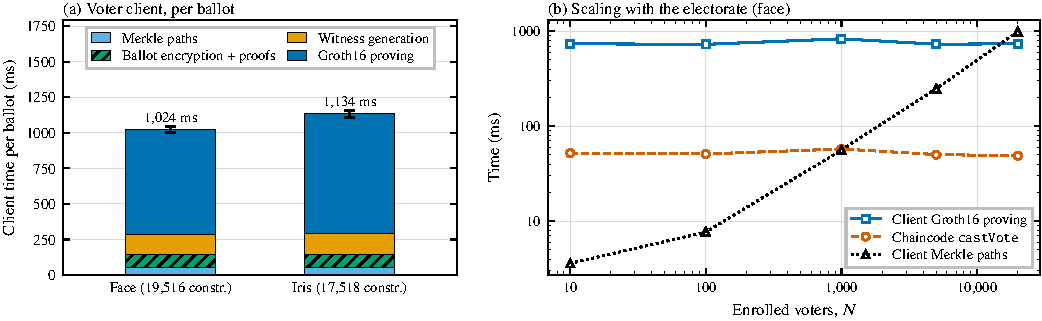
\includegraphics[width=0.9\textwidth]{figures/fig_supp_latency.pdf}
    \vspace{-4pt}
    \caption{(a)~Per-ballot client time by phase with 95\% CI on the total (20 ballots per modality, $N = 1{,}000$); (b)~face proving, chaincode \texttt{castVote}, and client Merkle-path time versus electorate size (log--log).}
    \label{fig:supp-latency}
\end{figure*}

\section{Circuit Architecture Details}
\label{sec:supp-circuit-details}

\subsection{Circuit Signals and Interfaces}
\label{sec:supp-signals}
Table~\ref{tab:circuit-signals} lists the signal interface of \texttt{FaceAuth} and \texttt{IrisAuth} (\texttt{api-server/circuits/}). The public signals are exactly what the chaincode stores and checks; everything else stays in the voter's client.

\begin{table}[t]
\caption{Circuit Signal Specification for \texttt{FaceAuth} and \texttt{IrisAuth}}
\label{tab:circuit-signals}
\centering
\scriptsize
\setlength{\tabcolsep}{3pt}
\renewcommand{\arraystretch}{1.04}
\resizebox{\columnwidth}{!}{%
\begin{tabular}{@{}llllp{3.6cm}@{}}
\toprule
\textbf{Signal} & \textbf{Vis.} & \textbf{Type} & \textbf{Mode} & \textbf{Meaning / chaincode check} \\
\midrule
\texttt{valid}               & Output  & $\{1\}$        & Both & Matcher passed; must be 1 \\
\texttt{merkleRoot}          & Public  & $\mathbb{F}_p$ & Both & Voter-tree root $R$; equals on-chain root \\
\texttt{nullifier}           & Public  & $\mathbb{F}_p$ & Both & $\nu = \mathcal{H}_2(sk, \mathcal{E}_{\mathsf{id}})$; must be unused \\
\texttt{electionId}          & Public  & $\mathbb{F}_p$ & Both & $\mathcal{E}_{\mathsf{id}}$; equals $\mathrm{trunc}_{128}\mathsf{SHA256}(\mathcal{B}.\mathrm{id})$ \\
\texttt{voteBinding}         & Public  & $\mathbb{F}_p$ & Both & $\mathsf{vb}$; equals hash of the submitted ciphertexts \\
\texttt{sensorRoot}          & Public  & $\mathbb{F}_p$ & Both & Device-registry root; equals on-chain root \\
\midrule
\texttt{embedding[128]}      & Private & $\mathbb{Z}^{128}$ & Face & Attested live sample, $|a_k| < 2^{\nCoordBits}$ \\
\texttt{registeredEmbedding[128]} & Private & $\mathbb{Z}^{128}$ & Face & Enrolled template, $|b_k| < 2^{\nCoordBits}$ \\
\texttt{irisCodeLive[256]}   & Private & $\{0,1\}^{256}$ & Iris & Attested live code \\
\texttt{irisCodeRegistered[256]} & Private & $\{0,1\}^{256}$ & Iris & Enrolled code \\
\texttt{salt}, \texttt{secretKey} & Private & $\mathbb{F}_p$ & Both & Client-generated $s$, $sk$ \\
\texttt{pathElements/Indices[20]} & Private & $\mathbb{F}_p^{20}, \{0,1\}^{20}$ & Both & Voter-tree opening (booleanity enforced) \\
\texttt{sessionNonce}        & Private & $\mathbb{F}_p$ & Both & $r$ in $\mathcal{H}_2(\nu, r)$ \\
\texttt{sensorAx/Ay}         & Private & $\mathbb{F}_p^2$ & Both & Capture-device EdDSA public key \\
\texttt{sigR8x/R8y/S}        & Private & $\mathbb{F}_p^3$ & Both & Device signature \\
\texttt{sensorPath*[10]}     & Private & $\mathbb{F}_p^{10}, \{0,1\}^{10}$ & Both & Registry opening (booleanity enforced) \\
\bottomrule
\end{tabular}%
}
\end{table}

\subsection{Constraint Complexity Breakdown}
\label{sec:supp-constraints}
Table~\ref{tab:constraints} reports R1CS constraints per sub-circuit, each compiled in isolation with the production flags (\texttt{circom --O2}) and counted with \texttt{snarkjs r1cs info} by \path{api-server/circuits/measure_subcircuits.sh} (output \path{api-server/results/subcircuit_constraints.json}). Because \texttt{--O2} simplifies across template boundaries, the components sum to the full circuit within two constraints.

\begin{table}[t]
\caption{Measured R1CS Constraints per Sub-Circuit (\texttt{circom --O2})}
\label{tab:constraints}
\centering
\scriptsize
\setlength{\tabcolsep}{3pt}
\renewcommand{\arraystretch}{1.04}
\begin{tabular}{@{}lrrr@{}}
\toprule
\textbf{Sub-circuit} & \textbf{Each} & \textbf{Face} & \textbf{Iris} \\
\midrule
\texttt{PackedCoordHash(128,19)} (template, live) & \nHashConstraints{} & $\times 2$ & -- \\
\texttt{PackedBitsHash(256)} (template, live)         & \nPackedHash & -- & $\times 2$ \\
\texttt{SquaredCosineSimilarity(128)} (incl.\ range/sign) & \nCosConstraints{} & $\times 1$ & -- \\
\texttt{HammingDistance(256)} (incl.\ booleanity)     & \nHamming & -- & $\times 1$ \\
\texttt{MerkleTreeChecker(20)}                        & \nMerkleConstraints{} & $\times 1$ & $\times 1$ \\
\texttt{SensorAttestation(10)} (EdDSA + registry)     & \nAttestConstraints{} & $\times 1$ & $\times 1$ \\
\texttt{Poseidon(2)} (salt, commitment, nullifier)    & \nPoseidonTwo & $\times 3$ & $\times 3$ \\
\midrule
\textbf{Full circuit}                                 &       & \textbf{\nFaceConstraints} & \textbf{\nIrisConstraints} \\
\bottomrule
\end{tabular}
\end{table}

Within the face comparator, \nRangeConstraints{} of the \nCosConstraints{} constraints are the per-coordinate range checks (256 coordinates $\times$ \nRangePerCoord{} bits) that make the squared-cosine test sound; the remainder is $3n + 2 = 386$ multiplications, the \nDotBits-bit sign check and a \nCmpBits-bit comparison. The attested-enrollment circuit (\path{enroll_auth.circom}) reuses the range check, \texttt{PackedCoordHash} and \texttt{SensorAttestation} with the election slot fixed to $D_{\mathsf{enr}} = 2^{200}$: \nEnrollConstraints{} constraints in a $2^{\nEnrollDomainExp}$ domain. Sensor attestation is the largest single component, so the price of binding the live sample to a device is about \nAttestShare\% of the face circuit.

\subsection{Fixed-Point Quantization and Range Arithmetic}
Face embeddings are L2-normalized $\mathbf{v} \in \mathbb{R}^{128}$, quantized as $a_k = \lfloor \sigma v_k \rceil$ with $\sigma = \nSigma$, so $|a_k| \le \sigma < 2^{\nCoordBits}$. Inside the circuit, $\cos\theta \geq \tau$ is checked without division:
\begin{equation}
  \langle \mathbf{a}, \mathbf{b} \rangle \geq 0 \;\wedge\; \langle \mathbf{a}, \mathbf{b} \rangle^2 \cdot \tau_{\mathsf{den}} \;\geq\; \tau_{\mathsf{num}} \cdot \|\mathbf{a}\|^2 \cdot \|\mathbf{b}\|^2, \label{eq:cosine-constraint}
\end{equation}
with $(\tau_{\mathsf{num}}, \tau_{\mathsf{den}}) = (1225, 10^4)$ fixed as template parameters ($\tau = 0.35$). The field is BN254's scalar field, $p \approx 2.19 \times 10^{76}$. Soundness over $\mathbb{F}_p$ requires that no intermediate wraps around $p$. This holds only because every coordinate of \emph{both} vectors is range-checked to $(-2^{\nCoordBits}, 2^{\nCoordBits})$: then $|\langle \mathbf{a}, \mathbf{b}\rangle|, \|\mathbf{a}\|^2, \|\mathbf{b}\|^2 < 128 \cdot 2^{\nTwoCoordBits} = 2^{\nDotBits}$, both sides of Eq.~\eqref{eq:cosine-constraint} are below $2^{2 \cdot \nDotBits} \cdot 2^{14} = 2^{\nCmpBits}$ (as $\tau_{\mathsf{num}} \le \tau_{\mathsf{den}} < 2^{14}$), and \texttt{GreaterEqThan(\nCmpBits)} compares the true integers. An honest quantizer alone does not suffice, since the prover chooses the witness. The non-negativity test (a \nDotBits-bit decomposition of the dot product) is needed because squaring accepts $\cos\theta \le -\tau$; without it the negated template passes (attack A5).

\emph{Packed hashing.} $\mathcal{H}_{\text{pack}}$ maps each coordinate to $u_k = a_k + 2^{\nCoordBits} \in [0, 2^{\nRangePerCoord})$ and packs 12 of them per field element, $e_j = \sum_{i<12} u_{12j+i} \, 2^{\nRangePerCoord i} < 2^{240} < p$, then hashes the 11 elements with one Poseidon. The map is linear, so it costs no constraints, and it is injective exactly when every $u_k$ lies in its slot, which the range checks above enforce for both vectors. Without them, moving $2^{\nRangePerCoord} c$ out of slot $i$ and $c$ into slot $i+1$ leaves $e_j$ unchanged; choosing $c$ from an attacker's face yields a template with the victim's digest that points at the attacker (attack A24).
For the iris channel, Hamming distance is linear over boolean-constrained bits,
\begin{equation}
  \mathsf{HD} = \sum_{j=0}^{255}(a_j + b_j - 2a_jb_j) < 123, \label{eq:hd}
\end{equation}
with the threshold again a template parameter.

\subsection{Metric and Dimensionality Baselines}
\label{sec:supp-euclidean-derivation}

The main manuscript's Euclidean comparison (Section~\ref{M-subsec:eval_baseline}) uses a sound squared-Euclidean comparator (\path{api-server/circuits/baselines/euclidean.circom}) with the same per-coordinate range checks as \texttt{SquaredCosineSimilarity} and the equivalent threshold $\|\mathbf{a}-\mathbf{b}\|^2 \le (2-2\tau)\sigma^2$ for unit vectors, a template constant whose value does not change the constraint count. Table~\ref{tab:supp-euclidean-baseline} lists the measured components (\texttt{measure\_subcircuits.sh}, \texttt{circom --O2}) and the resulting full-circuit costs.

\begin{table}[h]
\centering
\caption{Metric and Dimensionality Baselines: Measured Components and Full-Circuit Cost (Face)}
\label{tab:supp-euclidean-baseline}
\setlength{\tabcolsep}{3.5pt}
\renewcommand{\arraystretch}{1.1}
\resizebox{\columnwidth}{!}{%
\begin{tabular}{lcrrr}
\toprule
\textbf{Configuration} & \textbf{EER (\%)} & \textbf{Hash} & \textbf{Comparator} & \textbf{Full circuit} \\
\midrule
PCA-128, cosine (deployed) & \textbf{\nLfwEer} & \nHashConstraints{} & \nCosConstraints{} & \textbf{\nFaceConstraints} \\
PCA-128, Euclidean        & \nLfwEer{} & \nHashConstraints{} & \nEuclidConstraints{} & \nFullEuclid{} \\
PCA-96, cosine            & 0.27 & \nHashNinetySix{} & \nCosNinetySix{} & \nFullCosNinetySix{} \\
PCA-64, cosine            & 0.52 & \nHashSixtyFour{} & \nCosSixtyFour{} & \nFullCosSixtyFour{} \\
PCA-64, Euclidean         & 0.52 & \nHashSixtyFour{} & \nEuclidSixtyFour{} & \nFullEuclidSixtyFour{} \\
\bottomrule
\end{tabular}%
}
\end{table}

EER is measured on LFW with the deployed ArcFace embedding (\path{api-server/benchmark/face_sweep_insightface.json}); for unit vectors, cosine and Euclidean distance rank pairs identically, so each configuration's two metrics share one EER. \emph{Hash} is one \texttt{PackedCoordHash}($d$, 19) and \emph{Comparator} the range-checked metric, both measured in isolation. The first row is the compiled production circuit. The others substitute their measured components into it: $\text{Full} = \nFaceConstraints + 2(\text{Hash} - \nHashConstraints) + (\text{Comparator} - \nCosConstraints)$, because the template is hashed twice, enrolled and live. Every other sub-circuit (membership, attestation, nullifier) operates only on fixed-size digests and is independent of $d$ and the metric. Range checks cost \nRangePerCoord{} constraints per coordinate for either metric, so they dominate both comparators and the metric changes the full circuit by \nEuclidSaveShare\%, while each output dimension costs about \nPerDim{} constraints (\nChunkedPerDim{} with per-coordinate Poseidon chunks, \nChunkedHash{} per 128-D hash). With its public signals, the production circuit fits a $2^{\nDomainExp}$ FFT domain.

\section{Security Proofs}
\label{sec:supp-security-proofs}

This appendix gives the full arguments behind Section~\ref{M-sec:security} of the main manuscript. We use its notation: $\mathcal{H}_k$ is Poseidon of arity $k$, $\mathcal{H}_{\text{pack}}$ the packed template hash, $C = \mathcal{H}_2(\mathcal{H}_2(\mathcal{H}_{\text{pack}}(\mathbf{b}_{\text{reg}}), s), sk)$ the enrolled leaf, $\nu = \mathcal{H}_2(sk, \mathcal{E}_{\mathsf{id}})$ the nullifier, $\mathsf{vb}$ the vote binding, and $\mathsf{sr}$ the sensor-registry root. A ballot is $\beta = (\Pi, x, E(\mathbf{v}), \boldsymbol{\pi}^{\mathsf{val}}, \pi^{\Sigma})$ with public statement $x = (R, \nu, \mathcal{E}_{\mathsf{id}}, \mathsf{vb}, \mathsf{sr})$. The chaincode accepts $\beta$ for ballot $\mathcal{B}$ iff (V1)~$\mathsf{Groth16.Vfy}(\mathsf{vk}, x, \Pi) = 1$; (V2)~$R$ is the root of the on-chain commitment list; (V3)~$\mathcal{E}_{\mathsf{id}} = \mathrm{trunc}_{128}(\mathsf{SHA256}(\mathcal{B}.\mathrm{id}))$; (V4)~$\mathsf{sr}$ is the root of the on-chain sensor registry; (V5)~$\mathsf{vb} = \mathrm{trunc}_{248}(\mathsf{SHA256}(\mathcal{B}.\mathrm{id} \| E(\mathbf{v})))$; (V6)~every $\pi^{\mathsf{val}}_j$ and $\pi^{\Sigma}$ verifies with context $\mathcal{B}.\mathrm{id}\|\nu$ under the on-chain key $h$; and (V7)~$\nu$ is unused. The relation $\mathcal{R}$ proven by $\Pi$ is the conjunction of the constraints of Section~\ref{M-sec:protocol_construction}-C.

\subsection{Merkle Binding (Lemma~\ref{M-lem:merkle-binding})}
\label{sec:supp-proof-merkle-binding}

\begin{lemma}
\label{lem:supp-merkle-binding}
Let $R$ be the root of a depth-$L$ Poseidon tree over leaves $\{C_1, \ldots, C_m\}$ padded with zero-subtree digests. Given an opening $(C^\ast, (\sigma_\ell, d_\ell)_{\ell<L})$ with every $d_\ell \in \{0,1\}$ that hashes to $R$ and $C^\ast \notin \{C_i\}$, one can compute a collision for $\mathcal{H}_2$ in $O(L)$ time.
\end{lemma}

\begin{proof}
Let $u_0 = C^\ast$ and $u_{\ell+1} = \mathcal{H}_2(\mathsf{sw}_{d_\ell}(u_\ell, \sigma_\ell))$, where $\mathsf{sw}_0(a,b) = (a,b)$ and $\mathsf{sw}_1(a,b) = (b,a)$. Since $d_\ell \in \{0,1\}$, the bits $(d_\ell)$ name a leaf position $\iota$; let $w_\ell$ be the honest node on the path from leaf $\iota$, with $w_0 = C_\iota$ (or the zero leaf) and $w_L = R = u_L$. Because $u_0 \neq w_0$, there is a largest $\ell^\ast < L$ with $u_{\ell^\ast} \neq w_{\ell^\ast}$ and $u_{\ell^\ast+1} = w_{\ell^\ast+1}$. The two input pairs at level $\ell^\ast$ differ in the path coordinate and hash to the same value: a collision. If some $d_\ell \notin \{0,1\}$, the argument fails. For the root's children $(y_0, y_1)$ and any $u_{L-1}$, the prover sets $\sigma = y_0 + y_1 - u_{L-1}$ and $d = (y_0 - u_{L-1})/(\sigma - u_{L-1})$, so circomlib's \texttt{Switcher} outputs exactly $(y_0, y_1)$. This is attack A1, which the booleanity constraint $d_\ell(d_\ell - 1) = 0$ rules out.
\end{proof}

\subsection{Eligibility Soundness (Theorem~\ref{M-thm:eligibility})}
\label{sec:supp-proof-eligibility}

\paragraph{Game $\mathsf{Elig}$} The challenger runs setup, enrolls honest voters (keeping their credentials), and registers honest capture devices. $\mathcal{A}$ may corrupt voters (receiving their credentials), steal any honest voter's credential file, request device attestations for presentations of its choice (at most $q$ of which are \emph{non-genuine}, i.e., not a live presentation of the enrolled owner of the credential later used), and submit ballots. $\mathcal{A}$ wins if the ledger accepts a ballot whose extracted credential is honest and for which no genuine presentation of its owner was attested for that election and nullifier.

\begin{theorem}
\label{thm:supp-eligibility}
$\Pr[\mathcal{A} \text{ wins } \mathsf{Elig}] \leq \varepsilon^{\mathsf{ks}}_{\mathsf{G16}} + 4\,\mathbf{Adv}^{\mathsf{CR}}_{\mathsf{Pos}} + \mathbf{Adv}^{\mathsf{EUF}}_{\mathsf{EdDSA}} + q \cdot \mathsf{FAR}_\delta$.
\end{theorem}

\begin{proof}
Let $\beta^\ast$ be the winning ballot. By knowledge soundness in the AGM (A1), an extractor recovers a witness $w$ with $(x^\ast, w) \in \mathcal{R}$, except with probability $\varepsilon^{\mathsf{ks}}_{\mathsf{G16}}$. Consider the extracted values.

\emph{Enrolled leaf.} The witness opens leaf $C$ to $R$ with boolean directions, and (V2) fixes $R$ to the on-chain root. By Lemma~\ref{lem:supp-merkle-binding}, $C$ is an enrolled leaf, except with probability $\mathbf{Adv}^{\mathsf{CR}}_{\mathsf{Pos}}$.

\emph{Enrolled template.} The witness opens $C = \mathcal{H}_2(\mathcal{H}_2(\mathcal{H}_{\text{pack}}(\mathbf{b}_{\text{reg}}), s), sk)$. Since $C$ is an honest voter's leaf and packing is injective on the range-checked coordinates (see \emph{Match}), an extracted $(\mathbf{b}_{\text{reg}}, s, sk)$ other than the one enrolled yields a Poseidon collision, so $\mathbf{b}_{\text{reg}}$ is that voter's enrolled template, except with probability $\mathbf{Adv}^{\mathsf{CR}}_{\mathsf{Pos}}$.

\emph{Enrolled by the person captured.} Every face leaf entered the tree through \texttt{register}, which verifies $\pi_{\mathsf{enr}}$: by the same extraction, collision and EUF-CMA steps as below, the leaf's template is one a registered kiosk signed for that NID with domain $D_{\mathsf{enr}}$, which no vote signature carries since $\mathcal{E}_{\mathsf{id}} < 2^{128}$ (attacks A25--A27). Supervision ties that capture to the NID holder.

\emph{Registered device.} The witness opens $\mathcal{H}_2(A_x, A_y)$ to $\mathsf{sr}$, and (V4) fixes $\mathsf{sr}$. By the lemma again, $(A_x, A_y)$ is a registered device key, except with probability $\mathbf{Adv}^{\mathsf{CR}}_{\mathsf{Pos}}$.

\emph{Attested capture.} The EdDSA constraints verify a signature under that key on $m = \mathcal{H}_3(\mathcal{H}_{\text{pack}}(\mathbf{b}_{\text{live}}), \mathcal{E}_{\mathsf{id}}, \mathcal{H}_2(\nu, r))$. If no device signed $m$, this is an EUF-CMA forgery, with probability $\mathbf{Adv}^{\mathsf{EUF}}_{\mathsf{EdDSA}}$. Otherwise some device signed $m$. A witness $\mathbf{b}_{\text{live}}$ other than the sample that device signed, with the same $m$, would be a Poseidon collision in $\mathcal{H}_3 \circ \mathcal{H}_{\text{pack}}$, a fourth term $\mathbf{Adv}^{\mathsf{CR}}_{\mathsf{Pos}}$. So a device attested exactly $\mathbf{b}_{\text{live}}$ for this $\mathcal{E}_{\mathsf{id}}$ and nullifier. EUF-CMA is in the ROM with Poseidon as the signature hash; circomlib's verifier enforces $S$ below the subgroup order, rejects small-order keys, and checks the cofactor-cleared equation.

\emph{Match.} The comparator constraints hold with constants $(\tau_{\mathsf{num}}, \tau_{\mathsf{den}}) = (1225, 10^4)$ fixed in $\mathsf{vk}$, so no prover choice of threshold exists. Each coordinate is constrained to $(-2^{\nCoordBits}, 2^{\nCoordBits})$. Hence $|\langle \mathbf{a}, \mathbf{b} \rangle|, \|\mathbf{a}\|^2, \|\mathbf{b}\|^2 < 128 \cdot 2^{\nTwoCoordBits} = 2^{\nDotBits}$, and both sides of the squared inequality are below $2^{\nCmpBits} < p$. The integer inequality therefore equals the field inequality and \texttt{GreaterEqThan(\nCmpBits)} is sound. The constraint $\langle \mathbf{a}, \mathbf{b} \rangle \in [0, 2^{\nDotBits})$ excludes the negative branch $\cos\theta \leq -\tau$ that squaring would otherwise accept. Thus $\mathrm{dist}(\mathbf{b}_{\text{live}}, \mathbf{b}_{\text{reg}}) \leq \delta$.

Since $C$ is honest and, by the winning condition, the attested presentation was not a genuine presentation of $C$'s owner, it is one of the $q$ non-genuine presentations, each of which lands within $\delta$ with probability at most $\mathsf{FAR}_\delta$ (A5). A union bound over the events gives the claim.
\end{proof}

\begin{remark}
The bound is per election and grows linearly in $q$, so capture devices must rate-limit presentations. A5 must hold for the presentations the adversary \emph{chooses}, so $\mathsf{FAR}_\delta$ is the targeted, not the zero-effort, rate. An attacker who screens $K$ candidates offline and recruits the best lookalike reaches about $K$ times the zero-effort FAR with $q = 1$ (main manuscript, Fig.~\ref{M-fig:lookalike}); rate-limiting does not help there, and the threshold does. Artefact presentations of the victim (photos, replays, masks) are addressed only by the device's PAD (main manuscript, Section~\ref{M-sec:limitations}).
\end{remark}

\subsection{One Vote per Credential (Theorem~\ref{M-thm:antireplay})}
\label{sec:supp-proof-antireplay}

\begin{proof}
Suppose two ballots for the same ballot $\mathcal{B}$ are accepted whose extracted leaves are equal, $C^{(1)} = C^{(2)}$. By (V3) both use the same $\mathcal{E}_{\mathsf{id}}$. Without (V3) the prover could choose any $\mathcal{E}'_{\mathsf{id}}$ and obtain a fresh $\nu' = \mathcal{H}_2(sk, \mathcal{E}'_{\mathsf{id}})$ (attack A3). If the extracted keys are equal, $\nu^{(1)} = \nu^{(2)}$ and (V7) rejects the later transaction. Fabric's MVCC validation (Assumption~\ref{M-asm:fabric}) ensures this holds even for concurrent submissions, since both read and write the key \texttt{NULLIFIER}$\|\nu$. If the keys differ, then $C^{(1)} = C^{(2)}$ yields $\mathcal{H}_2(h^{(1)}, sk^{(1)}) = \mathcal{H}_2(h^{(2)}, sk^{(2)})$ with distinct inputs, a Poseidon collision. Extraction failures add $\varepsilon^{\mathsf{ks}}_{\mathsf{G16}}$.
\end{proof}

\subsection{Ballot Integrity (Theorem~\ref{M-thm:integrity})}
\label{sec:supp-proof-integrity}

\begin{proof}
(a)~\emph{Well-formedness.} For each $j$, $\pi^{\mathsf{val}}_j$ is a disjunctive Chaum--Pedersen proof that $(c_{1,j}, c_{2,j})$ encrypts $0$ or $1$; $\pi^{\Sigma}$ proves $\log_G \sum_j c_{1,j} = \log_h (\sum_j c_{2,j} - G)$, i.e., the vector sums to~1. Both are Fiat--Shamir transforms of special-sound $\Sigma$-protocols whose challenge hashes the public key, the statement and the context; in the ROM, an accepting proof for a false statement occurs with probability at most $q_H/n$ for $q_H$ oracle queries and group order $n$~\cite{Bernhard2012}. Without $\pi^{\Sigma}$, a vector of all ones passes every $\pi^{\mathsf{val}}_j$ (attack A11).

(b)~\emph{Non-malleability.} Let an honest voter publish $\beta = (\Pi, x, E, \ldots)$, and let $\mathcal{A}$ get $\beta' = (\Pi', x', E', \ldots)$ accepted with $\nu' = \nu$ and $E' \neq E$. By (V5), $\mathsf{vb}' = \mathsf{vb}$ would require a SHA-256 collision, so $x' \neq x$. The verification equation depends on $\mathsf{vb}$: the setup adds one constraint per public input, so the public-input polynomials are linearly independent, as Groth16's soundness proof assumes, and each has a non-zero verification-key point (we checked that changing an otherwise unused public input invalidates a snarkjs proof). The circuit's $\mathsf{vb}^2$ is a defensive measure only. Since $x'$ is a statement for which $\mathcal{A}$ saw no proof, weak simulation extractability (A1) extracts a witness with $\mathcal{H}_2(sk', \mathcal{E}_{\mathsf{id}}) = \nu$ and $sk'$ opening an enrolled leaf. Then either $sk' = sk$, so $\mathcal{A}$ inverted $\nu$ or $C$ (preimage resistance), or $sk' \neq sk$ gives a Poseidon collision. Proof re-randomisation does not help: it yields proofs for the same $x$, i.e., the honest ballot itself, already consumed by (V7) (attack A7). Conversely, reusing $E$ under a different nullifier $\nu'$ requires $\pi^{\mathsf{val}}$ for context $\mathcal{B}.\mathrm{id}\|\nu'$, i.e., new proofs for the honest ciphertexts. By special soundness this either reveals their randomness, contradicting DL, or is a forgery bounded as in~(a) (attack A12).
\end{proof}

\subsection{Ballot Privacy and Unlinkability (Theorem~\ref{M-thm:anonymity})}
\label{sec:supp-proof-anonymity}

\paragraph{Game $\mathsf{Priv}_b$} This is a swap game, weaker than BPRIV~\cite{Bernhard2015} because the tally is identical for both values of $b$, so no tally simulator is needed. $\mathcal{A}$ controls the gateway, the RA after enrollment, every capture device and every voter except two honest voters $V_0, V_1$ enrolled by the challenger. $\mathcal{A}$ picks vote vectors $\mathbf{v}_0, \mathbf{v}_1$. The challenger casts $\mathbf{v}_b$ for $V_0$ and $\mathbf{v}_{1-b}$ for $V_1$, interacting with $\mathcal{A}$'s devices as the protocol prescribes. $\mathcal{A}$ also corrupts a set $S$ of at most $t-1$ trustees and plays their part in the DKG. The honest trustees decrypt only the aggregates, whose totals are identical for $b = 0, 1$. $\mathcal{A}$ outputs $b'$. Unlinkability is the analogous game in which the challenger casts for $V_b$ in a second election after $\mathcal{A}$ has seen $V_0$'s ballot in the first.

\begin{proof}
Hybrids, from $\mathsf{Priv}_0$:
$\mathcal{G}_0'$: the honest trustees' partial decryptions are computed without their shares. From $T_j$ we know $x\hat{c}_{1,j} = \hat{c}_{2,j} - T_jG$, and the $t-1$ corrupt values $D_{m,j}$ are also known. These $t$ points of a degree-$(t-1)$ polynomial in the exponent determine every honest $D_{k,j}$ by Lagrange interpolation, and the DLEQ proofs are simulated in the ROM. This step is identical up to the ROM simulation, and $x$ is then used only through $h$. The $t-1$ corrupt shares are independent of $x$ (Shamir secrecy). For the DDH reduction below to embed its instance in $h$, the DKG must be simulatable, which holds for the variant of~\cite{Gennaro2007}; with joint-Feldman DKG this is the unbiased-key assumption stated in the main text.
$\mathcal{G}_1$: Groth16 proofs of the two challenge ballots are produced by the simulator, using the trapdoor that exists only inside this reduction. This is identical, by perfect ZK.
$\mathcal{G}_2$: the $\Sigma$-protocol proofs are simulated by programming the random oracle. The distance is at most $q_H(k+1)/n$, which is negligible.
$\mathcal{G}_3$: each of the $2k$ challenge ciphertexts is replaced by $E(0)$. The distance is at most $2k \cdot \mathbf{Adv}^{\mathsf{DDH}}$ by a standard hybrid, since the proofs no longer use the plaintext or the randomness.
In $\mathcal{G}_3$ the challenge ballots depend on $b$ only through $(\nu_0, \nu_1)$, the device inputs $\mathcal{H}_2(\nu_i, r_i)$, and the voters' enrolled leaves. With Poseidon modelled as a random oracle, $\nu_i = \mathcal{H}_2(sk_i, \mathcal{E}_{\mathsf{id}})$ is uniform and independent of $C_i$ unless $\mathcal{A}$ queries $(sk_i, \cdot)$, which happens with probability at most $q_H/2^{252}$. The gateway, RA and devices never receive $sk_i$: the RA receives $C_i$, the gateway receives $\beta$, and devices receive $\mathcal{H}_2(\nu_i, r_i)$ for fresh 248-bit $r_i$. So the challenge ballots are identically distributed for $b = 0, 1$ up to these events, and running the hybrids backwards reaches $\mathsf{Priv}_1$. Summing: $|\Pr[b'=1 \mid b=0] - \Pr[b'=1 \mid b=1]| \leq 2k \cdot \mathbf{Adv}^{\mathsf{DDH}} + \mathsf{negl}(\lambda)$. For unlinkability, the same argument applies with $\mathcal{E}_{\mathsf{id}} \neq \mathcal{E}'_{\mathsf{id}}$: $\nu$ and $\nu'$ are independent uniform values in the ROM. This holds only because no per-voter constant is public. Were the biometric hash $h_i$ a public input, it would link all of a voter's ballots (attack A4).
\end{proof}

\paragraph{Scope} The theorem says nothing about network metadata seen by the gateway, about the modality (separate trees), or against $t$ or more colluding trustees, who could decrypt individual ballots.

\subsection{Universal Verifiability (Proposition~\ref{M-prop:verif})}
\label{sec:supp-proof-verifiability}

\begin{proof}
An auditor reads every accepted ballot from the ledger and re-runs (V1)--(V6) using only $\mathsf{vk}$, the on-chain commitment and sensor lists, and the ballot record. It recomputes $h = \sum_{k\in\mathsf{QUAL}} A_{k0}$ and each verification key $h_k = \sum_{i\in\mathsf{QUAL}}\sum_\ell k^\ell A_{i\ell}$ from the on-chain dealings. It also computes $\hat{C}_j = \sum_i E(v_{i,j})$. For each published total it checks at least $t$ partial decryptions from distinct trustees, each with a Chaum--Pedersen proof of $\log_G h_k = \log_{\hat{c}_{1,j}} D_{k,j}$; the challenge hashes $(h_k, \hat{c}_{1,j}, D_{k,j}, \text{commitments})$ and the context $\mathcal{B}.\mathrm{id}\|j\|k$. Finally it checks that $\hat{c}_{2,j} - \sum_k \lambda_k D_{k,j} = T_jG$. If every proof is sound, $D_{k,j} = x_k\hat{c}_{1,j}$, so the interpolation equals $x\hat{c}_{1,j}$ and $T_j$ is the true total. Any false $T'_j$ therefore needs an accepting proof of a false statement, contradicting special soundness in the ROM. The chaincode performs exactly these checks in \texttt{publishTally} before recording the result (write-once, closed ballots only). \texttt{POST /tally/verify} repeats them off-chain. Inflated totals, under-threshold tallies and partial decryptions under shares outside the DKG are rejected (attacks A19--A21).
\end{proof}

\subsection{Coercion Under Observed Capture (main manuscript, Section~\ref{M-sec:coercion})}
\label{sec:supp-proof-coercion}

\begin{remark}[JCJ Deniability under Observed Capture]
\label{prop:coercion-impossibility}
If a coercer watches the voter present a trait to the capture device, the voter cannot fake a credential: an accepted proof needs a live sample within $\delta$ of the enrolled template, and any other presentation is either rejected or visibly different to the coercer, except with probability about $\mathsf{FAR}_\delta$. Deniable credentials therefore require that capture be unobserved, e.g., in a polling booth.
\end{remark}

\begin{proof}[Argument]
A JCJ-style fake credential must produce an accepted ballot indistinguishable to a coercer who observes the presentation. By Theorem~\ref{thm:supp-eligibility}, an accepted ballot requires an attested sample within $\delta$ of the template enrolled in the credential's leaf. If the voter presents their own trait, the coercer observes it and learns that the credential is genuine. If the voter presents anything else, it matches the enrolled template with probability at most $\mathsf{FAR}_\delta$ per presentation, or is rejected by PAD. A credential enrolled with a fake template cannot be created after enrollment, because new leaves enter only through the RA. So no unobservable fake credential exists, except with probability $\mathsf{FAR}_\delta + \mathsf{negl}(\lambda)$. Remote receipt-freeness therefore needs a mechanism outside the biometric check, which this work does not provide.
\end{proof}



\section{The Iris Variant: A Negative Result}
\label{sec:supp-iris}

The main manuscript evaluates face only. The prototype also implements an iris variant on the same protocol; this appendix reports it for completeness, and it carries no soundness claim.

\paragraph{Encoding and circuit} The 196,608-bit Daugman-style IrisCode (2-D Log-Gabor, phase-quantized) is reduced to 256 bits by mask-aware uniform striding. \texttt{iris\_auth.circom} packs the 256 boolean bits into 32 bytes for a $\text{Poseidon}_8 \rightarrow \text{Poseidon}_4$ commitment and evaluates Eq.~\eqref{eq:hd}, which enforces $\mathsf{HD} \le 122$ ($\mathsf{HD}/256 < 0.478$). With the same membership, nullifier and attestation sub-circuits it has \nIrisConstraints{} constraints (Table~\ref{tab:constraints}), against $\approx 5.9 \times 10^5$ for a Hamming comparator alone over the raw code. Each circuit-level attack of the main manuscript's Table~\ref{M-tab:attack_suite} is also run, and rejected, against this circuit.

\paragraph{Latency} Under the protocol of the main manuscript's Table~\ref{M-tab:combined_metrics} (20 ballots, $N = 1{,}000$): witness generation $\nIrisWitnessMs \pm \nIrisWitnessCi$\,ms, Groth16 proving $\nIrisProveMs \pm \nIrisProveCi$\,ms, client total $\nIrisClientMs \pm \nIrisClientCi$\,ms; device signing $\nIrisSignMs \pm \nIrisSignCi$\,ms; Groth16 verification $\nIrisVerifyMs \pm \nIrisVerifyCi$\,ms and \texttt{castVote} $\nIrisCastVoteMs \pm \nIrisCastVoteCi$\,ms. The proving key is \nIrisKeyMB\,MB.

\paragraph{Accuracy} On CASIA-Iris-Thousand (6,000 genuine / 6,000 impostor pairs), the EER is 46.29\% for the full code and 48.09\% for the deployed 256-bit code, with FAR 45.70\% and FRR 50.03\% at the circuit's threshold: near chance, so no meaningful eligibility bound follows.

\paragraph{Gabor Bit-Salience Masking (GBSM)} The 196,608-bit IrisCode (512$\times$64 normalized iris, three Log-Gabor wavelengths, two phase bits each) must be reduced to $d$ bits for the circuit. The deployed pipeline uses mask-aware uniform striding. GBSM instead scores each bit position by its empirical phase stability across repeated captures of the same eye (the ``fragile bits'' idea of~\cite{Hollingsworth2009}) and keeps the $d$ most stable positions. Both feed the same 256-bit Hamming comparator (778 constraints), so the comparison is purely about accuracy.

\paragraph{Results (CASIA-Iris-Thousand, 6,000 genuine / 6,000 impostor pairs)} With classical integro-differential segmentation, GBSM-256 reaches 48.68\% EER (FAR 48.48\%, FRR 48.90\% at the deployed threshold), against 48.09\% for striding and 46.29\% for the full code, i.e., all near chance. Because even the full code is near chance, bit selection cannot be the bottleneck; the likely cause is the classical segmentation stage upstream. We therefore do not propose GBSM. A deployable iris channel needs a stronger (e.g., fine-tuned deep) segmenter, after which bit selection would have to be re-derived and re-evaluated.


\section{Face Model and Encoding Comparison}
\label{sec:supp-face-models}

We ran the identical protocol (same LFW split and pairs) with three face pipelines: the deployed InsightFace \texttt{buffalo\_l} (SCRFD detection, five-point alignment, ArcFace R50; \texttt{run\_face\_eval.sh insightface}), the FaceNet baseline on a BlazeFace crop without landmark alignment (\texttt{deployed}, the prototype's first pipeline), and DeepFace's re-implementation of ArcFace with RetinaFace alignment (\texttt{ArcFace}). Every LFW image was embedded by all three; 39,726, 39,715 and 39,727 of the 39,733 sampled CelebA images were embedded, respectively.

\begin{table}[h]
\centering
\caption{LFW EER (\%) with 95\% Pair-Bootstrap CIs, Same Pairs for All Rows}
\label{tab:supp-face-models}
\setlength{\tabcolsep}{3pt}
\resizebox{\columnwidth}{!}{%
{\footnotesize
\begin{tabular}{lccc}
\toprule
\textbf{Encoding} & \textbf{\shortstack{ArcFace\\(InsightFace)}} & \textbf{FaceNet} & \textbf{\shortstack{ArcFace\\(DeepFace port)}} \\
\midrule
Raw (512 / 128 / 512-D) & 0.13 [0.05, 0.23] & 4.75 [4.37, 5.14] & 6.10 [5.61, 6.58] \\
PCA-64              & 0.52 [0.38, 0.65] & 4.38 [4.02, 4.78] & 6.78 [6.28, 7.28] \\
SOPQ-64             & 0.58 [0.42, 0.75] & 4.72 [4.31, 5.11] & 6.88 [6.39, 7.33] \\
PCA-96              & 0.27 [0.18, 0.38] & 4.38 & -- \\
PCA-128             & \textbf{\nLfwEer} [\nLfwEerLo, \nLfwEerHi] & -- & -- \\
\midrule
CelebA, PCA-64      & 4.52 & 8.09 & -- \\
\bottomrule
\end{tabular}}}
\end{table}

\paragraph{Findings} The trained weights matter more than the architecture's name: the DeepFace port of ArcFace is $\nDeepfaceRatio\times$ worse than InsightFace's original model at full dimension (\nDeepfaceEer\% vs.\ \nRawEer\%), even with a comparable aligner, and worse than FaceNet. A check on 200 random LFW images found that RetinaFace returns a different face first, rather than the centred, labelled one, in only 1\% of images, so face selection does not explain the gap. The embeddings' rank determines what reduction costs: 99\% of FaceNet's variance lies in 58 components and PCA-64 is lossless there (SOPQ is significantly worse, 0.33 points, CI [0.08, 0.57]), whereas both 512-D ArcFace embeddings are full-rank (375 components for InsightFace), so every reduction costs accuracy and PCA and SOPQ are statistically indistinguishable at 64-D (0.07 points, CI [$-0.10$, 0.25]). We therefore deploy InsightFace ArcFace with PCA-128 at $\tau = 0.35$, chosen on validation identities against a lookalike attacker by the rule of the main manuscript (Section~\ref{M-subsec:eval_encoding}).

\section{Template-Inversion Risk}
\label{sec:supp-inversion}

We assess what an adversary recovers if a template \emph{witness} leaks from the voter's client (side channel, client compromise, implementation bug). This is outside the threat model of the main manuscript's Section~\ref{M-sec:security}, but template protection is expected to address it~\cite{ISO24745}.

An attacker holding a leaked normalized PCA-128 template and the public projection $(\mathbf{W}, \boldsymbol{\mu})$ rescales it by the typical training norm and inverts, $\hat{\mathbf{v}} = \mathbf{W}^T(c\,\hat{\mathbf{z}}) + \boldsymbol{\mu}$. Because ArcFace is full-rank, the 384-D complement is lost: on the 5,471 held-out LFW images the reconstruction has only $\nInvCos$ mean cosine similarity to the true 512-D embedding (FaceNet PCA-64: $0.9998$). It nevertheless verifies against raw embeddings of other images of the same person almost as well as a genuine sample does (EER \nInvEer\% vs.\ \nInvRawEer\%), so the projection offers no protection against impersonation with a leaked template (\path{model/pca_followup.py}).

This does not weaken the security theorems: only the commitment $C_i$ is published and the proof is zero-knowledge, so template confidentiality rests on Poseidon preimage resistance and on the voter's sealed credential file, not on irreversibility of the encoding.

\bibliographystyle{IEEEtran}
\bibliography{References}

\end{document}
